%%%%%%%%%%%%%%%%%%%%%%%%%%%%%%%%%%%%%%%%%%%%%%%%%%%%%%%%%%%%%%%%%%%%%%%%%%%%%%
%% Diagnosing Faults in Reinforcement Learning Simulators and World Models
%% with Canonical Polynomial Invariants -- VERIFICATION-ONLY COMPANION FILE
%%
%% This file is a trimmed extract of the full paper, released so that
%% verify_properties.py can check the reported numbers against the tables
%% and figures below without publishing the full manuscript here. It keeps
%% only: the title, the tables and figures, the small set of definitions
%% those checks and the verification appendix depend on, the reproducibility
%% statement, and the verification appendix itself. The introduction,
%% related work, methods, main discussion, abstract and author details have
%% been removed. See [full paper link/DOI] for the complete paper.
%%%%%%%%%%%%%%%%%%%%%%%%%%%%%%%%%%%%%%%%%%%%%%%%%%%%%%%%%%%%%%%%%%%%%%%%%%%%%%

\documentclass{article}
\usepackage{iclr2027_conference,times}

% Inlined from math_commands.tex so this file is self-contained.
\providecommand{\R}{\mathbb{R}}
\providecommand{\N}{\mathbb{N}}
\providecommand{\Z}{\mathbb{Z}}
\providecommand{\Q}{\mathbb{Q}}
\providecommand{\E}{\mathbb{E}}

\usepackage{hyperref}
\usepackage{url}
\usepackage{amsmath,amssymb,amsthm}
\usepackage{mathtools}
\usepackage{enumitem}
\usepackage{xcolor}
\usepackage{algorithm}
\usepackage{algpseudocode}
\usepackage{multirow}
\usepackage{graphicx}
\graphicspath{{figures/}}
\usepackage{tabularx}
\usepackage{array}

\newtheorem{theorem}{Theorem}
\newtheorem{proposition}{Proposition}
\newtheorem{lemma}{Lemma}
\newtheorem{corollary}{Corollary}
\newtheorem{definition}{Definition}
\newtheorem{assumption}{Assumption}
\newtheorem{remark}{Remark}

\newcommand{\Lip}{\mathrm{Lip}}
\newcommand{\NF}{\mathrm{NF}}
\newcommand{\Var}{\mathbf{V}}

\title{Diagnosing Faults in Reinforcement Learning Simulators and World Models with Canonical Polynomial Invariants \\[4pt] \large (Verification companion -- tables, figures and checks only)}

\date{}

\begin{document}

\begin{center}
{\Large\bfseries Diagnosing Faults in Reinforcement Learning Simulators and World Models with Canonical Polynomial Invariants}\\[8pt]
{\large Verification companion}
\end{center}

\begin{quote}
\noindent\emph{This document accompanies the code in this repository. It is
\textbf{not} the paper. It contains only the tables and figures reported in
the paper, the small number of definitions the automated checks in
\texttt{verify\_properties.py} and Appendix~\ref{app:verified} depend on, the
Reproducibility Statement, and the verification appendix describing how the
checks work. The abstract, introduction, related work, methods, main
discussion, remaining appendices and author details have been removed from
this file. The full paper is available at [full paper link/DOI].}
\end{quote}


\section{Tables and Figures}
\label{sec:floats}

\begin{table}[t]
\caption{Detection, localisation and attribution over fifteen faults and two
healthy controls, one draw per cell. Localisation is scored as exact set
agreement with the fault's known constraint locus, and \emph{n/a} marks a method
with no constraint to name or, for the paired difference test, a regime it
cannot run in. The screen appears at two units of replication, blocks cut from
each trajectory and whole trajectories under an exact permutation null. The
paired noiseless control column is an identity check rather than a false-alarm
rate; Figure~\ref{fig:calibration} measures the rate.}
\label{tab:e1}
\begin{center}
\small
\begin{tabular}{llcccc}
regime, noise & method & faults detected & false alarms & localised & attributed \\
\hline
\multirow{6}{*}{unpaired, $\sigma=0$}
  & MMD permutation      & $12/15$ & $1/2$ & n/a & n/a \\
  & KS $+$ Bonferroni    & $10/15$ & $1/2$ & n/a & n/a \\
  & MLP discriminator    & $12/15$ & $1/2$ & n/a & n/a \\
  & paired difference    & n/a     & n/a   & n/a & n/a \\
  & \textbf{algebraic, per block} & $\mathbf{15/15}$ & $\mathbf{0/2}$
    & $\mathbf{15/15}$ & $7/7$ \\
  & \textbf{algebraic, per trajectory} & $\mathbf{15/15}$ & $\mathbf{0/2}$
    & $\mathbf{15/15}$ & $7/7$ \\
\hline
\multirow{6}{*}{paired, $\sigma=0$}
  & MMD permutation      & $7/15$  & $0/2$ & n/a & n/a \\
  & KS $+$ Bonferroni    & $6/15$  & $0/2$ & n/a & n/a \\
  & MLP discriminator    & $8/15$  & $0/2$ & n/a & n/a \\
  & \textbf{paired difference} & $\mathbf{15/15}$ & $0/2$ & n/a & n/a \\
  & \textbf{algebraic, per block} & $\mathbf{15/15}$ & $0/2$
    & $\mathbf{15/15}$ & $7/7$ \\
  & \textbf{algebraic, per trajectory} & $\mathbf{15/15}$ & $0/2$
    & $\mathbf{15/15}$ & $7/7$ \\
\hline
\multirow{6}{*}{paired, $\sigma=10^{-3}$}
  & MMD permutation      & $7/15$  & $0/2$ & n/a & n/a \\
  & KS $+$ Bonferroni    & $7/15$  & $0/2$ & n/a & n/a \\
  & MLP discriminator    & $8/15$  & $0/2$ & n/a & n/a \\
  & \textbf{paired difference} & $\mathbf{15/15}$ & $\mathbf{0/2}$
    & n/a & n/a \\
  & algebraic, per block & $11/15$ & $0/2$ & $10/15$ & $2/7$ \\
  & algebraic, per trajectory & $12/15$ & $\mathbf{0/2}$
    & $\mathbf{12/15}$ & $2/7$ \\
\end{tabular}
\end{center}
\end{table}

\begin{figure}[t]
\begin{center}
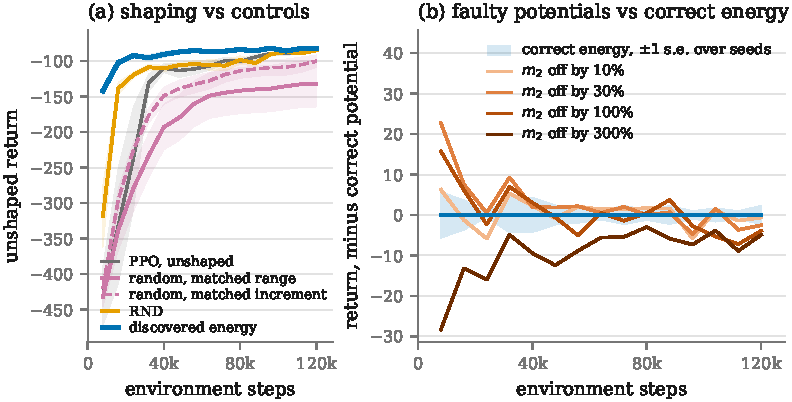
\includegraphics[width=\textwidth]{shaping_curves.pdf}
\end{center}
\caption{Acrobot swing-up, unshaped environment return, mean over five seeds.
\emph{(a)} The discovered energy leads unshaped PPO for the whole of the first
$40$k steps. The two random configurations, of the same degree and matched in
scale two different ways, each contain ten independent polynomial draws and five
PPO seeds per draw; all remain behind the discovered potential.
\emph{(b)} Each faulty potential is plotted against the correct one so that the
comparison is against seed-to-seed spread and not against the axis. Mass errors
of $10\%$, $30\%$ and $100\%$ stay inside the band; only $300\%$ leaves it, and
it leaves it downwards for most of training.}
\label{fig:shaping}
\end{figure}

\begin{table}[t]
\caption{Monomial dictionary size $M = \binom{n+d}{d}$. The support search
scales with $M$, not with $n$; degree is as important as dimension. A
degree-$1$ (linear) invariant class such as stoichiometric conservation is
tractable at any $n$ encountered in practice.}
\label{tab:dict}
\begin{center}
\begin{tabular}{r|rrrr}
$n$ & $d{=}1$ & $d{=}2$ & $d{=}3$ & $d{=}4$ \\
\hline
$4$  & $5$  & $15$  & $35$   & $70$   \\
$6$  & $7$  & $28$  & $84$   & $210$  \\
$8$  & $9$  & $45$  & $165$  & $495$  \\
$11$ & $12$ & $78$  & $364$  & $1365$ \\
$17$ & $18$ & $171$ & $1140$ & $5985$ \\
\end{tabular}
\end{center}
\end{table}

\begin{table}[t]
\caption{Deflating a single degree-$2$ invariant $g$ out of the degree-$\le d$
nullspace, $n = 4$. Orthogonal projection removes one direction at every
degree; normal-form reduction removes the entire filtered piece
$\langle g\rangle \cap \mathcal{P}_d$. The two agree only at $d = \deg g = 2$.}
\label{tab:lin-vs-gb}
\begin{center}
\begin{tabular}{cccc}
$d$ & multiples of $g$ present & projection removes & normal form removes \\
\hline
$2$ & $1$  & $1$ & $1$  \\
$3$ & $5$  & $1$ & $5$  \\
$4$ & $15$ & $1$ & $15$ \\
\end{tabular}
\end{center}
\end{table}

\begin{table}[t]
\caption{Nullspace deflation on Acrobot-v1, degree $\le 3$, $n=6$, $M=84$
monomials, single-energy passive trajectory, measured on sampled data and not
on the exact ideal. The $14$ trivial multiples vanish to machine precision
at every step size, being exact algebra; the energy direction vanishes only to
the integrator's drift floor, so admitting it requires a nullspace tolerance
above that floor. Sequential orthogonal projection of $g_1$ then $g_2$ removes
one direction in total, not two, for reasons given in the full paper's methods section. The last column is the residual of the single
surviving direction outside $\mathrm{span}\{E, 1\}$, and it is the column that
matters: at $\Delta t = 0.2$ the count collapses to $1$ just as it does at
$\Delta t = 0.002$, but the survivor is not the energy.}
\label{tab:deflation}
\begin{center}
\small
\begin{tabular}{cc|ccc|cl}
$\Delta t$ & tol & raw $d_{\mathrm{null}}$ & after projection
  & after normal form & residual & outcome \\
\hline
$0.2$   & $10^{-6}$  & $14$ & $13$ & $\mathbf{0}$ & --
  & energy below tolerance \\
$0.2$   & $10^{-4}$  & $15$ & $14$ & $\mathbf{1}$ & $6.2\times10^{-1}$
  & survivor is \emph{not} the energy \\
$0.05$  & $10^{-4}$  & $16$ & $15$ & $2$ & --
  & spurious direction admitted \\
$0.01$  & $10^{-6}$  & $15$ & $14$ & $\mathbf{1}$ & $1.6\times10^{-7}$
  & energy isolated exactly \\
$0.002$ & $10^{-6}$  & $15$ & $14$ & $\mathbf{1}$ & $4.9\times10^{-10}$
  & energy isolated exactly \\
\end{tabular}
\end{center}
\end{table}

\begin{table}[t]
\caption{An approximate reference set in place of the exact one, over the
fifteen catalogue faults and two healthy controls. \emph{(a)} The exact set with
every coefficient perturbed, at $\sigma = 0$; ranges are over five sign patterns
and both regimes, and the last column is the exact ideal-equality decision on the
same perturbed set. \emph{(b)} The set a numerical recovery returns from healthy
reference data, screened at the observation noise it was recovered at, against
the exact set on the same data; \emph{forced} removes the spectral-gap test so a
generator is returned whatever the conditioning. Deviations are relative and
gauge-fitted.}
\label{tab:approx}
\centering
\small
\begin{tabular}{lcccc}
\multicolumn{5}{l}{\emph{(a) Perturbed coefficients, $\sigma = 0$}} \\
\toprule
measured deviation & detected & localised & false alarms
  & $\langle G_\epsilon\rangle = \langle G\rangle$ \\
\midrule
$0$                                 & $15/15$    & $15/15$    & $0/4$   & yes \\
$\le 9.8\times10^{-5}$ (6 decades)  & $14$--$15/15$ & $14$--$15/15$ & $0/120$ & no  \\
$9.8\times10^{-4}$                  & $13$--$14/15$ & $13$--$14/15$ & $0/20$ & no \\
$9.9\times10^{-3}$                  & $9$--$13/15$  & $9$--$13/15$  & $0/20$ & no \\
$1.0\times10^{-1}$                  & $4$--$8/15$   & $3$--$5/15$   & $0/20$ & no \\
\bottomrule
\end{tabular}

\vspace{1.2ex}

\begin{tabular}{llcccc}
\multicolumn{6}{l}{\emph{(b) A recovered set against the exact one, at matched
observation noise}} \\
\toprule
reference set & $\sigma$ & generators & worst deviation & detected & localised \\
\midrule
exact     & $0$ & $8/8$ & $0$                  & $15/15$ & $15/15$ \\
recovered & $0$ & $8/8$ & $2.4\times10^{-8}$   & $15/15$ & $15/15$ \\
forced    & $0$ & $8/8$ & $2.4\times10^{-8}$   & $15/15$ & $15/15$ \\
\addlinespace
exact     & $10^{-8}$ & $8/8$ & $0$                & $14/15$ & $14/15$ \\
recovered & $10^{-8}$ & $7/8$ & $1.0\times10^{-5}$ & $14/15$ & $14/15$ \\
forced    & $10^{-8}$ & $8/8$ & $1.0\times10^{-5}$ & $15/15$ & $14/15$ \\
\addlinespace
exact     & $10^{-6}$ & $8/8$ & $0$                & $14/15$ & $14/15$ \\
recovered & $10^{-6}$ & $7/8$ & $7.0\times10^{-4}$ & $14/15$ & $14/15$ \\
forced    & $10^{-6}$ & $8/8$ & $7.0\times10^{-4}$ & $15/15$ & $14/15$ \\
\addlinespace
exact     & $10^{-4}$ & $8/8$ & $0$                & $13/15$ & $13/15$ \\
recovered & $10^{-4}$ & $6/8$ & $4.4\times10^{-4}$ & $5/15$  & $3/15$  \\
forced    & $10^{-4}$ & $8/8$ & $1.00$             & $12/15$ & $11/15$ \\
\bottomrule
\end{tabular}
\end{table}

\begin{figure}[t]
\begin{center}
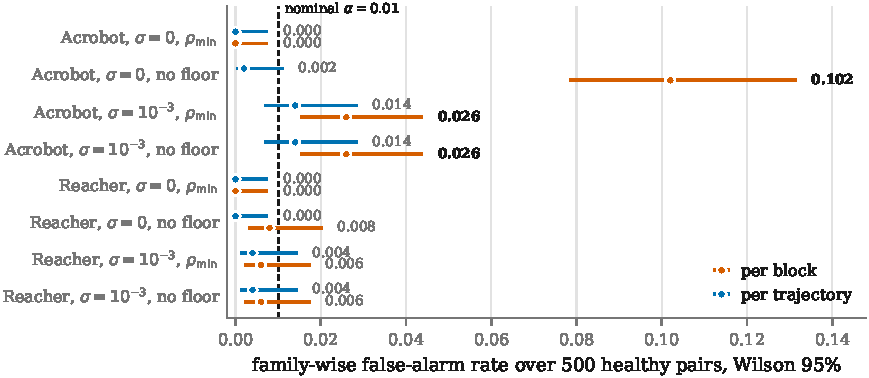
\includegraphics[width=\textwidth]{calibration.pdf}
\end{center}
\caption{Measured family-wise false-alarm rate over $500$ healthy-versus-healthy
comparisons per setting, against a nominal $\alpha = 0.01$, with Wilson $95\%$
intervals. Both configurations are the same model differing only by seed, so every
rejection is a false alarm by construction. $\rho_{\min}$ is the absolute
residual floor of this section and ``no floor'' removes it. Each pair is two
freshly drawn configurations with none reused, so the trials are independent and the
intervals describe the design. Three intervals lie
entirely to the right of the nominal line and all three are block-level and on
Acrobot; every trajectory-level interval covers it or sits below.}
\label{fig:calibration}
\end{figure}

\begin{table}[t]
\caption{Tier-A environments. All invariants listed are exact and hold under
arbitrary actuation unless marked \emph{(passive)}. ``Arity'' is the number of
state variables the invariant involves, which determines the size of the
variable subset that the recovery procedure must consider. The two environments in bold are the ones every
experiment in this paper runs on; the remaining four are stated to delimit the
class the construction applies to and carry no results here.}
\label{tab:tierA}
\begin{center}
\small
\begin{tabular}{lccl}
Environment & $n$ & deg & Invariants \\
\hline
Cartesian pendulum (DAE) & $4$ & $2$
  & $x^2{+}y^2{-}L^2$; $x\dot x{+}y\dot y$; energy \emph{(passive)} \\
\textbf{Acrobot-v1} & $6$ & $2$--$3$
  & $c_1^2{+}s_1^2{-}1$; $c_2^2{+}s_2^2{-}1$; energy \emph{(passive)};
    balance law \\
\textbf{Reacher-v4} & $\mathbf{11}$ & $1$--$2$
  & 2 unit-norm; $d_z{=}0$; 2 forward-kinematics \\
Free rigid body / attitude & $7$ & $2$
  & $\|q\|^2{-}1$; $\sum I_i\omega_i^2$, $\sum I_i^2\omega_i^2$
    \emph{(torque-free)} \\
Planar Kepler & $4$ & $2$
  & $x\dot y{-}y\dot x$; energy after lifting $r$ \\
Reaction network & $8$--$15$ & $\mathbf{1}$
  & moiety conservation, integer coefficients \\
\end{tabular}
\end{center}
\end{table}

\begin{table}[t]
\caption{The fifteen faults used in the fault-catalogue experiment, plus two healthy controls.
Every one is a mistake a real simulator or robot description has plausibly
carried. The \texttt{nips} Coriolis entry is not hypothetical but a variant
Gymnasium ships, so it is a structural fault with known ground truth that
no one wrote for this evaluation.}
\label{tab:faults}
\begin{center}
\small
\footnotesize
\begin{tabular}{@{}p{0.25\linewidth}@{}p{0.12\linewidth}@{}
p{0.40\linewidth}@{}>{\raggedright\arraybackslash}p{0.16\linewidth}@{}}
fault & category & description & must break \\
\hline
\texttt{acrobot\_m2\_1.3}   & parameter & second link mass $1.3$ not $1.0$
  & energy \\
\texttt{acrobot\_l1\_1.2}   & parameter & first link length $1.2$ not $1.0$
  & energy \\
\texttt{acrobot\_lc2\_0.6}  & parameter & second CoM at $0.6$ not $0.5$
  & energy \\
\texttt{acrobot\_I2\_1.5}   & parameter & second inertia $1.5$ not $1.0$
  & energy \\
\texttt{acrobot\_g\_9.81}   & parameter & gravity $9.81$ not $9.8$ & energy \\
\texttt{reacher\_l2\_0.13}  & parameter & $\ell_2 = 0.13$ not $0.11$
  & fk-$x$, fk-$y$ \\
\texttt{reacher\_l1\_0.09}  & parameter & $\ell_1 = 0.09$ not $0.10$
  & fk-$x$, fk-$y$ \\
\hline
\texttt{acrobot\_nips\_coriolis} & structural & the \texttt{nips} variant, a
  dropped Coriolis term & energy \\
\texttt{acrobot\_torque\_leak}   & structural & unmodelled constant torque
  $0.05$ & energy \\
\hline
\texttt{acrobot\_euler}     & numerical & explicit Euler substituted for RK4
  & energy \\
\texttt{acrobot\_dt\_0.2}   & numerical & the shipped $\Delta t = 0.2$, not
  the resolved $0.005$ & energy \\
\hline
\texttt{acrobot\_obs\_swap} & observation & $\sin\theta_1$, $\cos\theta_2$
  transposed & both unit-norm, energy \\
\texttt{acrobot\_obs\_unnormalised} & observation & $\cos\theta_1$ scaled by
  $1.02$ & unit-norm $\theta_1$, energy \\
\texttt{reacher\_dz\_offset} & observation & $10^{-3}$ $z$ leak into the
  fingertip vector & $d_z = 0$ \\
\texttt{reacher\_obs\_swap} & observation & $\cos\theta_2$, $\sin\theta_1$
  transposed & both unit-norm, fk-$x$, fk-$y$ \\
\hline
\shortstack[l]{\texttt{none\_acrobot}\\\texttt{none\_reacher}} & control & correct dynamics,
  reseeded & nothing \\
\end{tabular}
\end{center}
\end{table}

\begin{table}[t]
\caption{Fault-catalogue protocol. Every setting is fixed across all methods and
all faults. The baselines subsample because their cost is superlinear in the
sample count, whereas the screen's is not. The MMD permutation budget sets that
test's smallest attainable $p$ at $1/10001$, two orders below $\alpha$, so the
budget cannot be what decides its verdict; the kernel is built once and permuted
by index, which is what makes that budget affordable.}
\label{tab:e1protocol}
\begin{center}
\small
\begin{tabular}{ll}
setting & value \\
\hline
Acrobot trajectories & $8$ trajectories, $400$ steps, $\Delta t = 0.005$ \\
Reacher samples & $N = 4000$ poses, lengths scaled by $\ell_1$ \\
significance level $\alpha$ & $0.01$, Bonferroni corrected over $G_{\rm ref}$ \\
screen blocks & $32$ contiguous, $4$ per trajectory \\
screen trajectory units & $8$ per configuration, exact permutation null over
  $\binom{16}{8}$ splits \\
screen residual floor $\rho_{\min}$ & $10^{-8}$ \\
recovery spectral-gap threshold $\gamma$ & $0.1$ \\
attribution difference lag $k$ & $1$, $10$, $50$, $100$ \\
MMD & $n_{\rm sub} = 2000$, $10^4$ permutations, median-heuristic RBF \\
KS $+$ Bonferroni & $n_{\rm sub} = 2000$, asymptotic tail, per observation
  coordinate \\
MLP discriminator & $n_{\rm sub} = 3000$, two hidden layers of $64$, at most
  $300$ epochs \\
discriminator split & $50/20/30$ train/validation/test, early stopping on
  validation AUC, patience $20$ \\
discriminator decision rule & permutation $p < \alpha$ on held-out scores \\
paired difference & $32$ contiguous blocks, mean $|{\rm test} - {\rm ref}|$ per
  coordinate \\
paired difference null & the same statistic on a healthy paired pair,
  Bonferroni over coordinates \\
paired difference floor & $10^{-8}$, the same absolute floor the screen uses \\
\end{tabular}
\end{center}
\end{table}

\begin{table}[t]
\caption{Attribution under measurement noise: correct parameter named and
within $5\%$, out of seven parameter faults. The lag is the difference stride described in the full paper's methods section. Reacher's two faults are kinematic and use no
difference dictionary, which is why the count floors at two, not zero.}
\label{tab:attrnoise}
\begin{center}
\small
\begin{tabular}{r|cccc}
$\sigma$ & lag $1$ & lag $10$ & lag $50$ & lag $100$ \\
\hline
$0$        & $7$ & $7$ & $7$ & $7$ \\
$10^{-8}$  & $6$ & $6$ & $\mathbf{7}$ & $6$ \\
$10^{-7}$  & $2$ & $\mathbf{6}$ & $\mathbf{6}$ & $\mathbf{6}$ \\
$10^{-6}$  & $2$ & $2$ & $\mathbf{4}$ & $2$ \\
$10^{-5}$  & $2$ & $2$ & $2$ & $2$ \\
$10^{-4}$  & $2$ & $2$ & $2$ & $2$ \\
\end{tabular}
\end{center}
\end{table}

\begin{table}[t]
\caption{Smallest relative parameter error still rejected at $\alpha = 0.01$,
swept over $\{10^{-4}, 3\times10^{-4}, \dots, 0.3\}$. ``none'' means no swept
magnitude was rejected. The screen is at the bottom of the sweep on all four
constants without noise; under noise it separates by generator kind, staying
near there on Reacher's vanishing constraints and rising by two to three orders
on Acrobot's conserved one.}
\label{tab:floor}
\begin{center}
\small
\begin{tabular}{llcccc}
noise & constant & MMD & KS & discriminator & \textbf{screen} \\
\hline
\multirow{4}{*}{$\sigma = 0$}
 & Acrobot $m_2$    & $0.3$ & $0.3$ & $0.3$ & $\mathbf{\le 10^{-4}}$ \\
 & Acrobot $g$      & $0.3$ & $0.3$ & $0.3$ & $\mathbf{\le 10^{-4}}$ \\
 & Acrobot $l_{c2}$ & $0.3$ & $0.3$ & $0.3$ & $\mathbf{\le 10^{-4}}$ \\
 & Reacher $\ell_2$ & none & none & none & $\mathbf{\le 10^{-4}}$ \\
\hline
\multirow{4}{*}{$\sigma = 10^{-3}$}
 & Acrobot $m_2$    & $0.3$ & $0.3$ & $0.3$ & $\mathbf{0.1}$ \\
 & Acrobot $g$      & $0.3$ & $0.3$ & $0.3$ & $\mathbf{0.03}$ \\
 & Acrobot $l_{c2}$ & $0.3$ & $0.3$ & $0.3$ & $\mathbf{0.1}$ \\
 & Reacher $\ell_2$ & none & none & none & $\mathbf{10^{-3}}$ \\
\end{tabular}
\end{center}
\end{table}

\begin{table}[t]
\caption{True-positive rate over the fifteen catalogue faults as the
significance level sweeps twelve decades, scored at the trajectory unit. An
asterisk marks a level below the method's $p$-value floor, where a rate of
zero is arithmetic. The false-positive rate is $0.00$ over the two healthy
controls for every method and every level shown, which two controls bound only
at $[0, 0.66]$; the rate itself is measured in
Figure~\ref{fig:calibration}.}
\label{tab:roc}
\begin{center}
\small
\begin{tabular}{llcccc}
noise & $\alpha$ & MMD & KS & discriminator & \textbf{screen} \\
\hline
\multirow{6}{*}{$\sigma = 0$}
 & $10^{-12}$ & $0.00^{*}$ & $0.13$ & $0.53$ & $0.00^{*}$ \\
 & $10^{-6}$  & $0.00^{*}$ & $0.20$ & $0.53$ & $0.00^{*}$ \\
 & $10^{-4}$  & $0.33$ & $0.20$ & $0.53$ & $0.00^{*}$ \\
 & $10^{-3}$  & $0.33$ & $0.20$ & $0.53$ & $\mathbf{1.00}$ \\
 & $10^{-2}$  & $0.40$ & $0.40$ & $0.53$ & $\mathbf{1.00}$ \\
 & $0.05$     & $0.53$ & $0.40$ & $0.53$ & $\mathbf{1.00}$ \\
\hline
\multirow{6}{*}{$\sigma = 10^{-3}$}
 & $10^{-12}$ & $0.00^{*}$ & $0.20$ & $0.53$ & $0.00^{*}$ \\
 & $10^{-6}$  & $0.00^{*}$ & $0.27$ & $0.53$ & $0.00^{*}$ \\
 & $10^{-4}$  & $0.33$ & $0.27$ & $0.53$ & $0.00^{*}$ \\
 & $10^{-3}$  & $0.33$ & $0.27$ & $0.53$ & $\mathbf{0.80}$ \\
 & $10^{-2}$  & $0.40$ & $0.47$ & $0.53$ & $\mathbf{0.80}$ \\
 & $0.05$     & $0.53$ & $0.47$ & $0.53$ & $\mathbf{0.80}$ \\
\end{tabular}
\end{center}
\end{table}

\begin{table}[t]
\caption{Consistency weight against what it moves, paired within architecture,
data budget and seed, $12$ pairs per row against $\lambda = 0$. Ratios are
geometric means. The interval is a percentile bootstrap on the mean paired
difference in divergence horizon.}
\label{tab:lambda}
\begin{center}
\small
\begin{tabular}{lcccc}
$\lambda$ & val MSE & algebraic residual & horizon & $95\%$ interval \\
\hline
$10^{-3}$ & $1.000$ & $0.997$ & $-0.1$ & $[-0.5, +0.2]$ \\
$10^{-2}$ & $1.008$ & $1.000$ & $-1.3$ & $[-2.5, -0.1]$ \\
$10^{-1}$ & $1.036$ & $0.993$ & $-2.1$ & $[-6.0, +1.7]$ \\
$1$       & $1.574$ & $0.834$ & $-4.0$ & $[-8.2, +0.5]$ \\
$10$      & $7.540$ & $0.874$ & $-20.0$ & $[-24.4, -15.9]$ \\
$100$     & $64.16$ & $0.787$ & $-36.8$ & $[-44.7, -29.0]$ \\
\end{tabular}
\end{center}
\end{table}

\begin{table}[t]
\caption{Acrobot swing-up, PPO, five seeds, $120{,}000$ steps, unshaped
environment return, higher better. AUC is the mean return over a common step
grid. \emph{Spread} is the standard deviation of the deployed potential over
states a random policy visits, and \emph{step} the standard deviation of the
$\gamma\Phi(s') - \Phi(s)$ it hands the agent there, against an environment
reward of $-1$ per step. $\Delta$ is the AUC difference from the discovered
potential with a percentile bootstrap interval. The $p$ column flags detection
against \emph{none} only, uncorrected across conditions; five seeds against five
bottom out at $0.0079$ where ties do not force the asymptotic form. Random rows
give the mean and range of ten draw means, not a pooled seed-level interval or
$p$-value. RND runs at a single un-swept bonus coefficient.
Every faulty potential is recovered from a faulty system and gauged entirely
within it.}
\label{tab:shaping}

\small
\setlength{\tabcolsep}{2.5pt}

\begin{tabularx}{\textwidth}{@{}>{\raggedright\arraybackslash}X
  r r r r >{\raggedright\arraybackslash}X r@{}}
condition & AUC & final return & spread & step & $\Delta$ vs.\ discovered & $p$ \\
\hline
none (PPO)
  & $-147.8 \pm 28.4$
  & $-84.4 \pm 4.1$
  & & & $-56.5$ $[-81.6, -31.9]$
  & \\

rand. matched range
  & $-195.3$ $[-443.6, -126.7]$
  & $-132.7$ $[-416.5, -85.7]$
  & $5.75$ & $4.05$
  & $-104.0$ $[-352.3, -35.4]$
  & \\

rand. matched step
  & $-162.2$ $[-214.0, -135.1]$
  & $-99.1$ $[-169.6, -83.5]$
  & $1.06$ & $0.75$
  & $-70.9$ $[-122.7, -43.8]$
  & \\

RND \citep{burda2019rnd}
  & $-118.1 \pm 8.2$
  & $-85.8 \pm 3.1$
  & & &
  $-26.7$ $[-33.7, -19.0]$
  & $0.22$ \\

\textbf{discovered}
  & $\mathbf{-91.3 \pm 2.4}$
  & $-84.5 \pm 3.1$
  & $5.75$ & $0.75$
  & & $0.0079$ \\

faulty, $m_2$ $+10\%$
  & $-90.8 \pm 1.3$
  & $-83.7 \pm 2.2$
  & $6.07$ & $0.79$
  & $+0.5$ $[-1.5, +3.1]$
  & $0.0079$ \\

faulty, $m_2$ $+30\%$
  & $\mathbf{-88.6 \pm 1.6}$
  & $-85.3 \pm 3.1$
  & $6.71$ & $0.90$
  & $+2.7$ $[+0.4, +5.3]$
  & $0.0079$ \\

faulty, $m_2$ $+100\%$
  & $-90.8 \pm 1.9$
  & $-89.1 \pm 5.4$
  & $9.00$ & $1.49$
  & $+0.5$ $[-2.0, +3.2]$
  & $0.0079$ \\

faulty, $m_2$ $+300\%$
  & $-100.5 \pm 6.0$
  & $-88.1 \pm 4.0$
  & $15.68$ & $3.54$
  & $-9.2$ $[-15.2, -4.0]$
  & $0.0079$ \\
\end{tabularx}
\end{table}

\begin{figure}[t]
\begin{center}
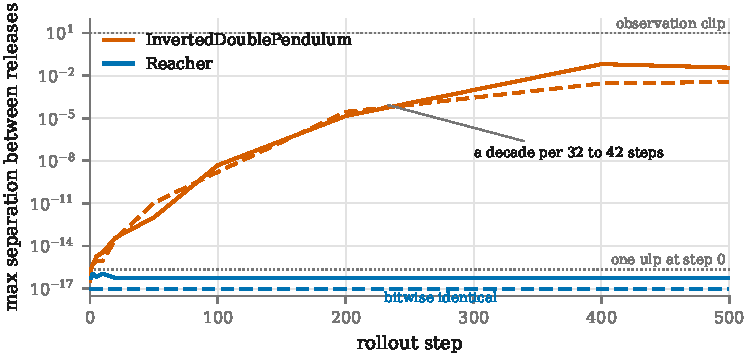
\includegraphics[width=\textwidth]{amplification.pdf}
\end{center}
\caption{Separation between two shipped releases running identical model files,
from a state both were handed identically. Colour is the environment and line
style the release pair. The chaotic environment climbs fourteen decades at a
constant rate from one unit in the last place, which is the signature of an
amplified rounding difference and not of a changed model; the non-chaotic one,
over the same release pairs and the same horizon, does not move. The lower
Reacher pair is bitwise identical at every step and is drawn on the axis
floor.}
\label{fig:amplification}
\end{figure}

\begin{table}[t]
\caption{Release audit. The reference system's energy drift sets the floor,
and the
smallest relative parameter error the screen localises tracks it. The first row
is the shipped configuration. Both parameters have spec value $1.0$, and
$\le 10^{-3}$ means every magnitude down to the bottom of the sweep was
localised.}
\label{tab:auditdt}
\begin{center}
\begin{tabular}{llll}
$\Delta t$ & reference energy drift & \texttt{LINK\_MASS\_2} &
  \texttt{LINK\_LENGTH\_1} \\
\hline
$0.2$ (shipped) & $3.55\times10^{-3}$ & $3\times10^{-2}$ & $10^{-1}$ \\
$0.05$          & $4.19\times10^{-6}$ & $\le 10^{-3}$ & $\le 10^{-3}$ \\
$0.01$          & $1.52\times10^{-8}$ & $\le 10^{-3}$ & $\le 10^{-3}$ \\
\end{tabular}
\end{center}
\end{table}

\section{Supporting Definitions}
\label{sec:supporting}

The items below are not the paper's methods section; they are the minimal
definitions that Appendix~\ref{app:verified} refers back to, kept here so
that appendix is self-contained.

\paragraph{Acrobot-v1 energy.} With the standard Gymnasium parameters
($m_1{=}m_2{=}1$, $l_1{=}l_2{=}1$, $l_{c1}{=}l_{c2}{=}\tfrac12$,
$I_1{=}I_2{=}1$, $g{=}9.8$) the total mechanical energy is \emph{exactly} the
degree-$3$ polynomial
\begin{equation}
\label{eq:acrobotE}
E = \tfrac{7}{4}\omega_1^2 + \tfrac{1}{2}c_2\omega_1^2
  + \tfrac{5}{4}\omega_1\omega_2 + \tfrac{1}{2}c_2\omega_1\omega_2
  + \tfrac{5}{8}\omega_2^2
  - \tfrac{147}{10}c_1 - \tfrac{49}{10}c_1c_2 + \tfrac{49}{10}s_1s_2
\end{equation}
in the observation vector $(c_1, s_1, c_2, s_2, \omega_1, \omega_2)$.

\paragraph{Reacher-v4 forward kinematics.} With observation
$(c_1, c_2, s_1, s_2, t_x, t_y, \omega_1, \omega_2, d_x, d_y, d_z)$, the
exact forward-kinematics identities are
\begin{equation}
\label{eq:reacherfk}
d_x + t_x - \ell_1 c_1 - \ell_2 (c_1c_2 - s_1s_2) = 0,
\qquad
d_y + t_y - \ell_1 s_1 - \ell_2 (s_1c_2 + c_1s_2) = 0.
\end{equation}
Link lengths are read from the environment XML rather than assumed; with the
standard $\ell_1 = 0.1$, $\ell_2 = 0.11$, \eqref{eq:reacherfk} is only
recoverable after nondimensionalisation, discussed in the full paper.


\begin{remark}[The reduced Gr\"obner basis is not a minimal generating set]
\label{rem:notminimal}
Uniqueness is often mistaken for minimality. It is not. For
$I = \langle y - x^2,\ z - x^3 \rangle$ (the twisted cubic), the reduced
Gr\"obner basis under grevlex is $\{\,x^2 - y,\ xy - z,\ y^2 - xz\,\}$: three
elements for an ideal with two generators, the third being an algebraic
consequence of the first two (verified symbolically,
Appendix~\ref{app:tc}). Consequently a loss of the form
$\sum_{p \in G} \|p(\cdot)\|^2$ does \emph{not} assign one penalty per
independent constraint. Separately, even a minimal generating set need not
have one generator per unit of codimension, since most varieties are not
complete intersections. Where minimality is genuinely required we obtain it
by an explicit extra step (interreduction, or minimal generators via the
degree-graded strand of a minimal free resolution for homogeneous ideals) and
we say so; we do not obtain it from canonicalisation.
\end{remark}

\begin{remark}[The tension between tolerating drift and resolving it]
\label{rem:tension}
An invariant-based shield must tolerate its integrator's drift, and a
drift diagnostic exists to resolve it, so the two pull in opposite directions.
On Acrobot at Gymnasium's $\Delta t = 0.2$ with RK4, relative energy drift over
a $40\,$s passive rollout is $6.5\times10^{-4}$, falling to $6.9\times10^{-7}$
at $\Delta t = 0.05$ and $2.2\times10^{-10}$ at $\Delta t = 0.01$
(Appendix~\ref{app:drift}). The same floor bounds \emph{discovery}: the energy
direction enters the numerical nullspace only once
the tolerance exceeds the drift, and a tolerance that loose already admits
spurious content. The usable window closes as $\Delta t$ coarsens, and on
Acrobot it has closed by the shipped step size. Discovering the conserved
quantity therefore requires re-integrating the environment more finely than it
ships. The full paper's shaping experiment runs into this directly: the potential must be
discovered on a re-integrated copy and then deployed on the environment as
distributed.
\end{remark}

\section*{Reproducibility Statement}

Code for every experiment is available at https://www.github.com/TesfayZ/algebraicRLtest.git. Every number in the paper's Experiments section and in Appendix~\ref{app:verified} below is produced by a script there; the mapping from result to script is in the accompanying README, and the checks of Appendix~\ref{app:verified} exit nonzero if any claim there has drifted from the text. This file is a trimmed, verification-only extract of the paper released alongside the code; it retains only the tables, figures and definitions the checks depend on. The full paper is available at [full paper link/DOI].

% Inlined from references.bib -- only the entry actually cited (in
% Table~\ref{tab:shaping}) is included, so this file is self-contained.
\begin{thebibliography}{1}

\bibitem{burda2019rnd}
Yuri Burda, Harrison Edwards, Amos Storkey, and Oleg Klimov.
\newblock Exploration by random network distillation.
\newblock In {\em International Conference on Learning Representations (ICLR)}, 2019.

\end{thebibliography}

\appendix

\section{Verified Environment and Algebraic Properties}
\label{app:verified}

\emph{This appendix is included in this repository's companion document for the sole purpose of documenting what \texttt{verify\_properties.py} checks and why. This file is not the paper: it has been stripped down to the tables, figures and the minimal supporting definitions the checks depend on. For the full paper, including the methods, experiments and discussion, see [full paper link/DOI].}

All statements below are outputs of the verification driver in the accompanying
repository (Python 3.14, SymPy $1.14$, NumPy $2.5$), which runs $145$ checks and
exits nonzero if any claim in this appendix has drifted from the text. Every
numerical check compares against the figure printed here to a relative
tolerance of $5\%$, rather than against an order-of-magnitude bound, so a value
that drifts inside its own order of magnitude still fails. The repository README
maps each claim to the script that establishes it. None is an experimental
result.

Six of the checks guard the diagnostic itself, not the environments. The
Acrobot energy exists twice in the codebase, once numerically and once
symbolically so that attribution can differentiate it with respect to physical
parameters, and a duplicated definition is where two things drift apart; the
check asserts they agree to $2.8\times10^{-14}$ over random states. The same is
asserted for Reacher's forward-kinematics template, which vanishes to
$8.9\times10^{-16}$ on generated poses. A third runs the full level-2 procedure
on a healthy system and asserts that the verdict is not \emph{parameter fault},
since a diagnostic that accuses correct software is worse than no diagnostic.
The remaining three assert that the trivial filtered piece has dimension $14$,
that the undeflated least-varying direction lies wholly inside it with zero
alignment to the energy, and that the deflated one aligns with the energy to
$1.0000$.

A further block of eight guards behaviour that a results table cannot see,
because each concerns a case the reported experiments do not visit. The two
conditions on a level-2 verdict are asserted separately, since a recovered
generator that is well separated but that no hypothesis fits must return
\emph{not explicable as a parameter fault} and not \emph{consistent with
specification}; the check builds exactly that case by perturbing an $m_2 = 1.3$
energy along a monomial outside the template's support. The residual floor is
asserted to be absolute by screening a $d_z$ leak of $10^{-30}$ and requiring
that it is \emph{not} flagged while a leak of $10^{-3}$ is, which is the
distinction a scale-relative floor cannot draw on a single-term generator.
The numerical nullspace of a $3 \times 10$ design matrix is asserted to have all
seven of its dimensions, and to satisfy $\Phi v = 0$ on each. And the random
control of the full paper's shaping experiment is asserted to have the same spread over the
state space as the energy, to one percent, so that ``matched in scale'' remains
a measured property of the potential actually deployed.

A last group covers quantities the results tables have no column for. The
shaping section's gauge is one: its recovered energy, its agreement with the
analytic form and the five targets $E^\star$ come out of the discovery step and
not out of the training run, so none of them is a column of the returns table
and each is recomputed and compared here. The chaotic growth rate is another.
Both the rate and the number of decades climbed are quoted in
the full paper's chaotic-amplification experiment and in Figure~\ref{fig:amplification}, and both are written
into the trace the figure is drawn from and read back, since a figure computed
only for a terminal is one that nothing can contradict. Table~\ref{tab:roc} is
compared cell by cell against the sweep that produced it, and its censoring
marks are derived from each method's $p$-value floor instead of trusted,
because a mark on the wrong row turns a measurement into arithmetic or the
reverse.

\paragraph{A model detail that determines everything else.} Gymnasium's Acrobot
offers two dynamics variants. The default, \texttt{book}, carries the term
$-m_2 l_1 l_{c2}\dot\theta_1^2\sin\theta_2$ in the second equation of motion;
the \texttt{nips} variant omits it. Only the former conserves the energy
\eqref{eq:acrobotE}. Under the latter, passive energy drift plateaus near
$1.7\times10^{-4}$ independently of $\Delta t$, which presents as an integrator
failure but is a model inconsistency, and every drift and balance number below
would be meaningless under it. The discrepancy is invisible until one measures
convergence order rather than drift magnitude, which is why the variant is
pinned explicitly rather than left at whatever the installed release defaults
to.

\subsection{Acrobot energy as a polynomial in the observation}
\label{app:acrobot}
Equation~\eqref{eq:acrobotE} is derived symbolically from the mass matrix and
potential, not asserted, and the derivation recovers exactly the eight
terms printed there. Over $2000$ uniformly random states the maximum discrepancy
between \eqref{eq:acrobotE} evaluated on the observation vector and the
mechanical energy $T + V$ evaluated in $(\theta,\omega)$ coordinates is
$1.14\times10^{-13}$, i.e.\ machine precision. The coefficient denominators are
$\{2,4,8,10\}$, so the largest is $10 \le Q_{\max} = 16$ and the invariant is
representable by snap-rounding without rescaling.

\subsection{Passive drift under RK4}
\label{app:drift}
Relative energy drift $|\Delta E| / |E_0|$ over a $40\,$s passive rollout from
$(\theta,\omega) = (0.1, -0.2, 0.3, -0.15)$: $6.51\times10^{-4}$ at
$\Delta t = 0.2$
(Gymnasium's default); $6.86\times10^{-7}$ at $\Delta t = 0.05$;
$2.20\times10^{-10}$ at $\Delta t = 0.01$. The implied convergence order is
$4.95$, consistent with RK4. This is the drift floor of
Remark~\ref{rem:tension}, and it is the quantity that bounds the resolution of
any diagnostic built on a conserved quantity.

\subsection{Power balance under torque}
\label{app:balance}
With $\tau = 1$, the mean residual of
$E(s') - E(s) - \Delta t\,\tau\,\omega_2$ over $200$ steps is
$2.48\times10^{-3}$ at $\Delta t = 0.05$, $1.06\times10^{-4}$ at
$\Delta t = 0.01$ and $6.12\times10^{-6}$ at $\Delta t = 0.002$; the ratio
residual$/\Delta t^2$ is $0.99$, $1.06$ and $1.53$ respectively, a spread of
$1.5\times$ over a $25\times$ range of step sizes, which confirms a first-order
identity with $O(\Delta t^2)$ discretisation error.

\subsection{The twisted cubic}
\label{app:tc}
For $I = \langle y - x^2,\ z - x^3\rangle$ the reduced Gr\"obner basis under
grevlex with $x > y > z$ is $\{x^2 - y,\ xy - z,\ y^2 - xz\}$. The ideal
generated by the first two elements equals the ideal generated by all three, so
the third is redundant as a generator: three basis elements for a two-generator
ideal. This witnesses Remark~\ref{rem:notminimal}.

\subsection{Deflation on Acrobot}
\label{app:deflation}
With $n = 6$ and $d = 3$ the dictionary has $M = \binom{9}{3} = 84$ monomials.
The degree-$\le 3$ filtered piece of $\langle g_1, g_2\rangle$ has dimension
$14$, namely the products $m \cdot g_j$ with $\deg m \le 1$ and
$j \in \{1,2\}$; adjoining the energy direction gives $15$. Reducing modulo the
reduced Gr\"obner basis of $\langle g_1, g_2\rangle$ sends all fourteen to zero
and leaves the energy direction non-zero, giving a deflated nullspace of
dimension $1$. That much is exact algebra and holds at any tolerance;
Table~\ref{tab:deflation} reports what happens on sampled trajectories, where
it does not.

\paragraph{Sequential projection saturates.} On the same system, projecting
$g_1$ out of the $14$-dimensional component and then $g_2$ out of the result
removes one direction in total, leaving $13$. Both generators carry the
constant term $-1$, so their coefficient vectors have inner product $1$, and
after the first projection $g_2$ no longer lies in the subspace. The control
case confirms that this is the cause, not a numerical artefact: for the
orthogonal generators $h_1 = xy$ and $h_2 = zw$ in $n = 4$ variables, whose
coefficient vectors have inner product $0$, the same sequential projection
removes one direction per generator as the informal argument predicts, taking
the degree-$\le 3$ component from $10$ to $8$. Normal-form reduction removes all
$14$ and all $10$ respectively, in both cases.

\subsection{Reacher forward kinematics and the units failure}
\label{app:reacher}
Over $5000$ random poses the maximum residual of \eqref{eq:reacherfk} is
$7.29\times10^{-17}$. In metres the coefficients are $1/10$ and $11/100$, with
denominators $10$ and $100$; at $Q_{\max}=16$ the second is not representable
and the invariant is not recoverable. Rescaling lengths by $\ell_1$ gives $1$
and $11/10$, with denominators $1$ and $10$, both admissible.

\end{document}